\documentclass[12pt]{article}

\usepackage[utf8]{inputenc}
\usepackage[czech]{babel}
\usepackage{graphicx}
\usepackage{wrapfig}  % balík na obtékání obrázku textem

\title{
\includegraphics[scale=0.3]{pic/FAV_cmyk.png} \hfill 
\includegraphics[scale=0.3]{pic/ZCU_cmyk.png} \\ \vspace{2cm} Sauron Gorthaur \\ Semestrální práce - HKUI}  % drobné znásilnění titulu práce, aby byla loga jakoby v záhlaví
\author{mr. Example}
\date{\today}
%\date{prvního října dva tisíce devatenáct}

% title, author a date využívá příkaz maketitle ke tvorbě titulní stránky, její podoba je dána typem dokumentu

\begin{document}
\maketitle
\thispagestyle{empty}
\newpage
\listoffigures

\tableofcontents
\newpage

\setcounter{page}{1}
\section{Životopis}
\begin{wrapfigure}{r}  % obrázek obtékaný textem (obrázek je vpravo, jakože right, proto 'r') ;)
    \centering
    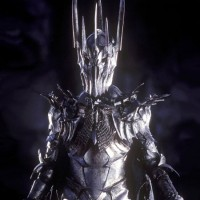
\includegraphics{pic/sauron-foto.jpg}
    \caption{Sauron v hmotné podobě.}
    % caption v prostředí figure zalistuje název obrázku pro případné generování automatického seznamu obrázků a doplní slovo 'Obrázek #' do popisu v závislosti na jazyku definovaném v documentclassu
    {\large{\textit{"Ash nazg durbatulûk, Ash nazg gimbatul, Ash nazg thrakatulûk, agh burzum-ishi krimpatul."} - Sauron}}  
    \label{fig:my_label} % label umožňuje odkaz na číslo obrázeku pomocí příkazu ref (viz další odstavec)
\end{wrapfigure}



\subsection{Počátek}
Sauron (viz. Obrázek~\ref{fig:my_label}) patřil k Aulëho lidu, projevoval se jako velký řemeslník. Sauron byl původem mnohem vyššího řádu než např. Gandalf nebo Saruman, a největší, nejnebezpečnější, a nejspolehlivější Melkorův služebník, jeho pobočník v Angbandu, a po jeho pádu sám Temný pán a Nepřítel.

Eru ponechal andělské duchy hrát Hudbu Ainur (Ainulindalë), kteří rozvíjeli téma zjevené samotným Eru. Melkor se však pokoušel zvýšit svou slávu ve své písni svými myšlenkami a ideami, které nebyly v souladu s původním Tématem Hudby. „… a rázem kolem něho vznikl nelad a mnozí, kteří zpívali blízko něho, propadli sklíčenosti, jejich myšlenky se narušily a jejich hudba zakolísala; někteří však začali ladit svou hudbu spíš podle něho než podle myšlenky, kterou měli zprvu.“

Melkorova disharmonie měla své strašlivé důsledky, jelikož Eru dovolil Ainur vykonat „Píseň Stvoření“, jako šablonu světa, který byl stvořen: „Zlo světa nebylo na poprvé ve velkém Tématu, ale vstoupilo s disharmonií Melkora.“ Sauron nebyl původcem disharmonie a nepochybně věděl víc o Hudbě než Melkor, jehož mysl byla vždy naplněna jeho vlastními plány a záměry. Zřejmě Sauron nebyl jedním z duchů, kteří okamžitě ladili svou Hudbu podle Melkora.

Brzy Melkorova disharmonie jako by byla ve válce s Tématem Eru - Hudba reprezentuje konflikt dobra a zla. Nakonec Eru píseň ukončil. Aby duchové viděli, co učinili, Eru učinil bytí Hudby. Tak byl stvořen vesmír Eä, ve kterém měl být konflikt dobra a zla rozhodnut. Eru umožnil duchům vstoupit do Eä. Mnoho tak učinilo a Sauron byl mezi nimi. Tím, že jim umožnil vstoupit do světa, umožnil jak velké zlo, tak velké dobro. 

\subsection{První věk}
Po vstupu do Eä na začátku času, se Valar a jejich Maiar pokusili vybudovat svět podle vůle Ilúvatara. Ve svém úsilí se Sauron projevil jako „velký řemeslník patřící k Aulëmu“. Jako ostatní Valar, Aulë učil své služebníky Maiar o struktuře, zákonech a podstatě světa a Sauron získal tuto znalost.

Uvnitř obrovských prostor Eä Valar zaměřili své úsilí na Ardu, Zemi, kde elfové a lidé budou žít. Ale Melkor, později známý jako Morgoth, také přišel do Ardy. Toužíc stát se svrchovaným pánem světa oponoval ostatním Valar, kteří zůstali věrní Ilúvatarovi a snažili se sledovat Stvořitelův plán. V této době Sauron podlehl Melkorově vlivu. Tolkien poznamenal, že Sauron obdivoval pořádek a koordinaci a nesnášel zmatek a neuspořádané třenice. Tak moc a vůle Melkora po nastolení pořádku v Ardě Saurona přitahovala.

Sauron měl podíl na všech činech Melkora na Ardě a byl jen o to méně zlý, že zpočátku sloužil jinému a ne sobě. Po jistou dobu zřejmě předstíral, že je věrným služebníkem Valar, zatímco předával Melkorovi informace o všem, co činili. Když Valar vytvořili říši Almaren, osvětlenou svitem Dvou lamp, Melkor o všem věděl, protože měl zvědy mezi Maiar a Sauron byl jejich náčelníkem.

Melkor zničil Almaren a Valar vytvořili novou zemi na Nejzazším Západě: říši Valinor. Valar ještě nevěděli o Sauronově zradě, a tak Sauron zůstal mezi nimi. Teprve později Sauron Valinor opustil a odešel do Středozemě, centrálního kontinentu Ardy. Od té chvíle byl Sauron definitivně na straně Melkora. Poté, co se přidal k Melkorovi ve Středozemi, prokázal, že je oddaným a schopným služebníkem, a Melkor mu svěřil správu své pevnosti Angband.

Ta nebyla po Druhé válce s Melkorem (brzy po procitnutí elfů) příliš prozkoumávána, takže Sauron nebyl dopaden. Po Melkorově návratu se stal jeho nejmocnějším sluhou, byl pánem mučení. Po bitvě Náhlého plamene ovládl Tol Sirion, kam se nastěhoval se svými vlkodlaky a kde věznil mimo jiné Finroda Felegunda a Berena, než byl nucen předat vládu nad věží Lúthien Tinúviel. Po Válce hněvu se Sauron zatoužil napravit a prosil Eönwëho, herolda Valar, o odpuštění, ten však neměl pravomoc odpustit bytosti vlastního řádu, a proto jej vyzval, aby se s ním vrátil do Amanu, kde předstoupí před Soudný kruh Valar. Sauron se však zalekl přísného trestu a raději zůstal ve Středozemi, kde se ukryl daleko na Východě. 

\subsection{Druhý věk}
Po pěti stoletích Druhého věku se Sauron znovu objevil. Rozhodl se stát vládcem Středozemě a podrobit si všechny její svobodné národy. Vzal na sebe nádherný vzhled a sám se nazýval „Annatarem, Pánem Darů“, vyslanec Valar a žák Aulëho (označoval se také jménem Aulendil, Aulëho přítel). Díky jeho hlubokým znalostem se Sauronovi podařilo získat důvěru elfích kovářů v Eregionu. Elfům se představil jako vyslanec Valar. Někteří elfové mu ovšem nedůvěřovali, mezi nimi zejména Galadriel a Gil-galad. Ale elfové v Eregionu neposlechli jejich varování.

Se Sauronovou pomocí elfští kováři vyrobili Prsteny moci, jež zadržovaly a posilovaly moc svých nositelů. Tři nejmocnější z nich vyrobil kovář Celebrimbor sám a věnoval je nejmocnějším z elfů - Gil-galadovi, Galadriel a Círdanovi. Ostatní Prsteny vyrobil Sauron. Devět z nich věnoval mocným vládcům lidí, protože lidé nejvíce touží po moci. Sedm prstenů obdrželi vládci trpaslíků (přičemž se praví, že sedmý, nejmocnější z nich přijal Durin, vládce Khazad-dûm, z rukou Celebrimbora, nikoli Saurona). Sauron však všechny oklamal a tajně v Hoře osudu v Mordoru vyrobil svůj vlastní, Jeden prsten, který poskytoval moc vládnout a zároveň i ovládat ostatní prsteny a jejich nositele podrobit Sauronově vůli. Prsteny moci však měly velkou moc a k jejich ovládání byl Sauron nucen vložit část své vlastní přirozené moci do Vládnoucího prstenu. Dokud byl ovšem držitelem Prstenu, jeho vlastní moc byla ještě zvětšena. Sauron nikdy nepředpokládal, že by někdo jiný než on získal a použil Jeden prsten.

Pokud by se tak stalo, nový vlastník Prstenu mohl (pokud by byl dost silný a mocný svou vlastní přirozeností) přemoci Saurona, stát se pánem všeho, co Sauron znal nebo učinil od vytvoření Prstenu, a tak ho svrhnout a usurpovat jeho místo. Byla zde ještě další slabina: pokud by byl Jeden prsten zničen, jeho moc by pominula, Sauronovo vlastní bytí by bylo zmenšeno do nicotnosti a on by byl snížen do pouhého stínu, pouhou vzpomínkou zlé vůle. Ale to on nikdy neuvažoval ani se toho nebál. Prsten byl nezničitelný jakýmkoli kovářským uměním menším než jeho vlastním. Byl neroztavitelný ohněm, kromě neuhasínajícího podzemního ohně, kde byl vytvořen, a ten byl přístupný jen v Mordoru. A v každém případě byl na Sauronově prstu.

Když si však Sauron Jeden prsten nasadil a pokusil se ovládnout elfy, důvtipný postřeh je varoval a oni si uvědomili jeho úmysly. Konečně poznali, kým je Annatar doopravdy a od té doby byl Sauron znám jako Temný pán Mordoru. Elfové sňali své Prsteny a už je nenosili ani neužívali, dokud Sauron vlastnil Jeden prsten. Trpaslíky se Sauronovi rovněž nepodařilo ovládat pomocí Sedmi, protože byli příliš nezlomní, takže na ně Prsteny měly jen malý vliv, leda že jim vnášely do srdce nepokoj a touhu po moci. Zato lidé se pomocí Devíti nechali snadno zotročit a stali se nazgûly, Prstenovými přízraky, nejstrašnějšími ze Sauronových služebníků. Když Sauron selhal v ovládnutí elfů, rozzuřil se a odpověděl vojenskou silou. Rozpoutal válku elfů se Sauronem a rychle si podrobil mnoho zemí. Tím začaly Temné roky. Dobyl Eregion a zabil Celebrimbora, obléhal Imlandris (Roklinku), sváděl boje s Morií a Lórienem a postupoval dál do Gil-galadovy říše. Vyzdvihl Barad-dûr, Temnou věž, postavil Morannon, Černou bránu Mordoru, aby zabránil možné invazi, a podrobil své moci zlé bytosti, které sloužily Morgothovi v Prvním věku (jako skřeti a trolové). Sauron také vládl lidem na Východě a Jihu. Prohlásil se Pánem země a králem lidí. Elfové však bojovali dál a s pomocí mocné armády númenorského krále Tar-Minastira zničili Sauronovu armádu a vytlačili ho do Mordoru. Númenorejci byli nejmocnějším královstvím své doby a když připluli se svým velikým vojskem, Sauronovi služebníci prchali. Sauron proto raději hledal cestu, jak prosadit své záměry lstí. Vzdal se králi a nechal se odvést na Númenor. Kde se díky svým hlubokým znalostem a lstivému našeptávání postupně stal z vězně královým rádcem a nakonec přiměl krále Ar-Pharazôna k útoku na Valinor. Valar požádali o pomoc Eru Ilúvatara a ten - jako odpověď na númenorejský útok - ostrov Númenor potopil a zničil Ar-Pharazônovu flotilu.

Sauron ve zkáze zahynul, ale jeho duch se vrátil do Středozemě, vytvořil si novou podobu a znovu se pokusil ovládnout Středozem. Narazil však na Dúnadany, kteří unikli ze zkázy Númenoru, a založili ve Středozemi Říše ve vyhnanství, Arnor a Gondor. Jelikož se Sauron bál síly Dúnadanů, pokusil se je zničit hned na začátku. Zaútočil na Gondor a dobyl Minas Ithil. Isildur unikl z města a odplul za svým otcem Elendilem po Anduině. Elendil uzavřel s Gil-galadem Poslední spojenectví elfů a lidí a vytáhl proti armádám Mordoru a Sauronovi.

Sauron byl Posledním spojenectvím v bitvě na Dagorladu poražen a ustoupil do Mordoru. Vojska Posledního spojenectví jej oblehla v Barad-dûr. Isildurův bratr Anárion během obléhání zahynul zasažen kamenem. Nakonec byl Sauron donucen vyjít ze své pevnosti a bojovat sám. Na svazích Hory osudu se střetl v souboji s Elendilem a Gil-galadem. V souboji všichni tři zahynuli. Isildur pak zlomeným Narsilem uťal Sauronovi Jeden prsten a Sauron ztratil svou podobu. Isildur si poté vzal Sauronův vládnoucí prsten jako náhradu za smrt otce a bratra. Jeden prsten však Isildura zradil a Isildur zahynul, když unikal přes Anduinu z bitvy na Kosatcových polích. Jeden prsten pak na dva a půl tisíc let zmizel, dokud ho v hlubinách Anduiny nenašel hobit Déagol, jemuž jej vzápětí násilím odebral jeho bratranec Sméagol. 

\end{document}


